\chapter{Analysis}
To test the hypothesis a closed loop system based on the Good Old Fashion Artificial Intelligence (GOFAI) environment interaction model \cite{Pfeifer2007} was developed (Figure \ref{fig:block_diagram}). In the following each block will be described with respect to functionality and interfaces.

\begin{figure}[htb]
	\begin{center}
		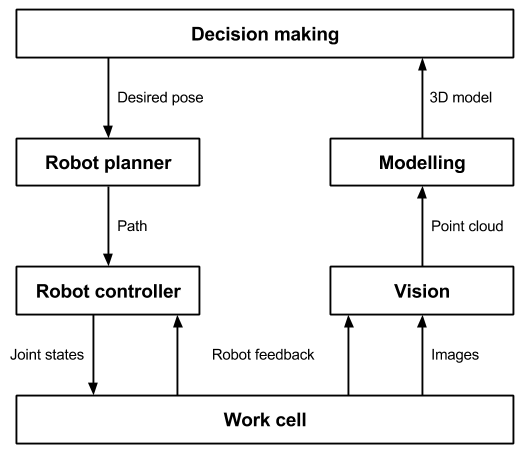
\includegraphics[scale=0.5,trim=0 0 0 0]{graphics/02_analysis/block_diagram.png}%trim=l b r t
		\caption{Block diagram of the eye-in-hand 3D reconstruction system.}
		\label{fig:block_diagram}
	\end{center}
\end{figure}

\subsection{Decision maker}
The desired pose is ‘hard-coded’ into the decision maker to capture the object from for example 24 discrete locations on a sphere. The captions are uniformly distributed to cover the entire object. When the robot is at rest in the desired pose a signal is sent to the vision block to capture the current view.

\subsection{Robot planner}
The robot planner executes the desired pose based on the PRM algorithm subject to the constraint that the camera always points to the center of the object being modelled. The robot planner is based on the Open Motion Planning Library (OMPL) which is integrated into the moveIt stack in ROS and collision checking is based on the a priori model of the work cell.

\subsection{Robot controller}
The robot controller further processes the path adding kinematics and time tessellation to meet velocity and acceleration constraints. The controller interpolates the joint states and handles closed loop control with feedback from the workcell. The robot controller is based on the control stack in ROS.

\subsection{Work cell}
The workcell contains a six degrees of freedom RX60 robot arm with a stereo camera mounted on the end effector. The work cell interface is based on a ROS node communicating with the robot and a node broadcasting data from the camera.

\subsection{Vision}
The vision module takes input from the stereo camera mounted on the end effector of the robot. The images are undistorted and rectified using calibration parameters obtained independently using the ROS calibration node. A disparity image is generated using the semiglobal block matching \cite{Hirschmuller2008}, and by using the obtained projective parameters the point cloud is obtained. The vision part will be implemented with a combination of built-in ROS nodes and homemade ROS nodes using the OpenCV library for image processing.

\subsection{Modelling}
The point clouds from the vision block are transformed to a common frame based on the robot pose and are then cropped, filtered and combined into one point cloud representing the sum of information about the object. Methods from Point Cloud Library (PCL) will be used for point cloud cropping, filtering and the assembly process. A wavelet based algorithm will be implemented for surface reconstruction according to \cite{Manson2008}.
